\chapter{Introduction}
\section{Introduction To Organisation}
I had my six months industrial training at DigiMantra Labs, IT Park, Ludhiana.
DigiMantra Labs is an IT company based in India. It was established in 2009. The CEO of this company is Mr. Sachin Khosla. DigiMantra mainly focus in development of preeminent Web, Mobile and Desktop solutions. It believes  in delivering quality and cater diversified niche of industries. DigiMantra have a proven track record of delivering high performance solutions to various big to small level industries. This company is aided by Government of India.\\\\
DigiMantra Labs is a customary participant of various important events like IndiaSoft, ICT – HongKong. It always look forward to build new relationships with like minded companies/ individuals. 
DigiMantra has a  team of young dynamic professionals formed by the group of engineers who have graduated from reputed Engineering Colleges. Their team is lead by professional who has worked with big products like Limewire, Trulia etc. 
\\\\
Good thing about DigiMantra is that it is driven by ethical values, energy to build great apps and determination to deliver the best. They are keen to provide out of box solutions to the client keeping the ‘cost to company’ aside.
 DigiMantra teams are trained to work under various software models such as Agile, Scrum etc. They make sure that they adhere to these standards so that they are able to deliver quality product 
 All the activities at office are closely monitored and recorded using CCTV cameras. We just ensure that your business plan is safe with us.
DigiMantra innovate and build our applications using latest technologies, which makes them fast, robust \& scalable. This company contributes to open source software by organizing / participating in OSS Camps.\\
Their expertise is in the following fields:-\\
\begin{itemize}
\item Enterprise Level Product Development 
\item Internet Tools including Viral campaigns, Affiliate Marketing solutions 
\item Mobile Application Development; iOS \& Android 
\item Cloud Computing Solutions – SaaS \& PaaS 
\item Website Development with Complete CMS and Social Networking Support 
\item User Experience \& Product Designing 
\item Social Media Applications \& Campaigning 
 \end{itemize}
\begin{figure}[h]
\centering 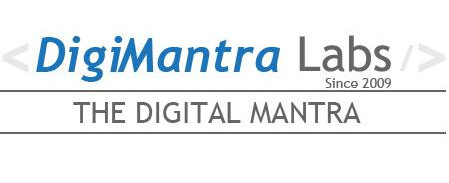
\includegraphics[scale=0.9]{image/digimantra.png}
\caption[GNDEC]{DigiMantra Labs Logo}
\end{figure}
DigiMantra believes that 'communication' is the foremost ingredient to make a project successful. It communicate with the clients on regular basis and using the dedicated VOIP lines and various other ways of communication. 
This company understand different needs of different customers and hence have custom solutions based on the requirement. Their onsite team facilitation is one such example.

%%%%%%%%%%%%%%%%%%%%%%%%%%%%%%%%%%%%%%%%%%%%%%%%%%%%%%%%%%%%%%%%%%%%%%%%%%%%%%%%%%%%%%%%%%%%%%%%%%%%%%%%%%%%%%%%%%%%%%%%%%%%%%%%%%%
\pagebreak
\section{Introduction to Project}

e-Notice App helps you access online notices on your phone. It is an online notice board maker
where a group of people can easily communicate with each other by sticking virtual notes. These
notes can have text, images or include online videos such as from YouTube.\\\\
The notice board has always been the place where staff/students gathers to get their latest release
of corporate news. eNotice brings the notice board to a virtual location where staff/students can
not only read notices, but immediately react and respond to them - from their own desks!
With this electronic notice and announcement system, notification alerts may be sent out notifying
staff and students that a new notice has been posted, where staff may know if it concerns him directly. In this
way, e-Notice also serves as a mailing list for all employees in the directory. This eliminates the
need to keep a separate mailing list which is hard to maintain due to the rapid movement of staff.\\ \\
These are the features that an eNotice App should have:
\begin{itemize}
\item An electronic dashboard board for disseminating information out to staff and students.
\item Notices can be posted, with response obtained instantly.
\item Staff or student can be notified of new postings via notification alert.
\item Notice administrator may push important notices in to selected staff's email.
\item Notice administrator may create any notice category.
\end{itemize}
The interface of this application is straightforward and takes you roughly a minute to get started.
Adding notes to board is easy, just click on the post notice button and enter the text. Users can view the post 
on the spot by having a notification alert in android phone.
Here registration is must for all the users having this application in order they want to have notification and staying stuned.\\ \\
This application can also acts as a market place and lets you advertise, for example, a room to
rent, a car for sale, a job opportunity, a house for sale, an upcoming event, an announcement, a
service, and so on.
\\
This application creates interactive notice boards online. You can customize boards with a
custom background, title and background images. It allows users to add sticky notes with text,
images and videos. You can set preferences on who can edit and view the board. Facility of drag
and drop notes anywhere on the board is available. Users can sign using their Google accounts /
Facebook Account and can share boards with others.

%%%%%%%%%%%%%%%%%%%%%%%%%%%%%%%%%%%%%%%%%%%%%%%%%%%%%%%%%%%%%%%%%%%%%%%%%%%%%%%%%%%%%%%%%%%%%%%%%%%%%%%%%%%%%%%%%%%%%%%%%%%%%%%%%%%
\pagebreak
\section{Project Category (Mobile Application) }

"e-Notice App" is a mobile application i.e an Internet based Mobile application. A mobile application is a computer program designed to run on smartphones, tablet computers and other mobile devices.
Apps are usually available through application distribution platforms, which began appearing in 2008 and are typically operated by the owner of the mobile operating system, such as the Apple App Store, Google Play, Windows Phone Store, and BlackBerry App World.\\\\
Mobile apps were originally offered for general productivity and information retrieval, including email, calendar, contacts, and stock market and weather information. However, public demand and the availability of developer tools drove rapid expansion into other categories, such as mobile games, factory automation, GPS and location-based services, banking, order-tracking, ticket purchases and recently mobile medical apps. The explosion in number and variety of apps made discovery a challenge, which in turn led to the creation of a wide range of review, recommendation, and curation sources, including blogs, magazines, and dedicated online app-discovery services.
\\ \\
Mobile application development is the process by which application software is developed for low-power handheld devices, such as personal digital assistants, enterprise digital assistants or mobile phones. These applications can be pre-installed on phones during manufacturing, downloaded by customers from various mobile software distribution platforms, or delivered as web applications using server-side or client-side processing (e.g. JavaScript) to provide an "application-like" experience within a Web browser.\\ \\
 Application software developers also have to consider a lengthy array of screen sizes, hardware specifications and configurations because of intense competition in mobile software and changes within each of the platforms. Mobile app development has been steadily growing, both in terms of revenues and jobs created. 
The popularity of mobile apps has continued to rise, as their usage has become increasingly prevalent across mobile phone users.

%%%%%%%%%%%%%%%%%%%%%%%%%%%%%%%%%%%%%%%%%%%%%%%%%%%%%%%%%%%%%%%%%%%%%%%%%%%%%%%%%%%%%%%%%%%%%%%%%%%%%%%%%%%%%%%%%%%%%%%%%%%%%%
\pagebreak
\section{Objective}

The proposed system's objectives are to overcome all the limitations and drawbacks of the
existing system. The online ‘eNotice’ application is user-friendly android application. The main
objective of the application is its simplicity of design and ease of implementation that shows and
helps to collect most of the information about events going on in college premises. The interface
will be very user-friendly. \\ \\
The main objectives of the proposed system can be enumerated as follows:
\begin{itemize}
\item Faster dissemination of notices regarding education, technical events, cultural events.
\item Any lost/found going out in college.
\item Easy way to broadcast your message.
\item Helps you to be updated with whats going on in College.
\item Good way to advertise about Tuitions/ Coaching and Courses.
\item User can also follow a group notice board.
\end{itemize}

%%%%%%%%%%%%%%%%%%%%%%%%%%%%%%%%%%%%%%%%%%%%%%%%%%%%%%%%%%%%%%%%%%%%%%%%%%%%%%%%%%%%%%%%%%%%%%%%%%%%%%%%%%%%%%%%%%%%%%%%%%%%%%%
\pagebreak
\section{Problem Formulation}

To develop a mobile application that will help you receiving the notices from the college, anywhere , anytime. Earlier their was problem that notices were pasted on notice board. If there is holiday on the next day, nobody will be able to read it. Moreover any update on website is also very difficult. Everyone feels lazy to go and update the website data. The more easy way is, just type in message sitting wherever and post by pressing a button. It will notify all the staff and students, registered with that application. \\

%%%%%%%%%%%%%%%%%%%%%%%%%%%%%%%%%%%%%%%%%%%%%%%%%%%%%%%%%%%%%%%%%%%%%%%%%%%%%%%%%%%%%%%%%%%%%%%%%%%%%%%%%%%%%%%%%%%%%%%%%%%%%%%%%
\pagebreak
\section{Identification of Need}
\begin{enumerate}
\item As we discussed earlier that manual maintenance of a notices is a tedious
job. So to enhance the ease of working, we go for this package.

\item Giving  the facility to convey messages to all students anytime and anywhere.

\item Making students updated about all the events and activities going on in the college.

\item The student will not require to stand in the crowd to see the notice.
There wil be no issue of fighting in order to see the notice first. Everyone is first to see that notice inside thier own mobile phone 
anywhere and anytime.
\item The least but most important it saves time.

\item Utilizing less man power. As there are many persons involved in circulating the message. With this application, only one person is required to post the notice. Rest of the man power is saved in the entire process.

\end{enumerate}

%%%%%%%%%%%%%%%%%%%%%%%%%%%%%%%%%%%%%%%%%%%%%%%%%%%%%%%%%%%%%%%%%%%%%%%%%%%%%%%%%%%%%%%%%%%%%%%%%%%%%%%%%%%%%%%%%%%%%%%%%%
\pagebreak
\section{Existing System}
Currently our college has manual system of putting notices on notice board. Its outdated now.
As nobody has a time to stand in rush in order to read the notices on noticeboard.

\textbf{\emph{Limitations of Existing System:}}
\begin{enumerate}
\item \textbf{\emph{Order of Data}}: Notice can get out of order in traditional notice board system. If
someone accidentally puts some data in the wrong place, it can lead to lost data. Automated
notice management systems allow users to quickly check whether information already exists
somewhere in the system, which helps avoid problems like redundant data.
\item \textbf{\emph{Complexity}}: Automated system is less complex than manual system of handling notices, which can make
it easier for untrained people to access and manipulate data. Anyone having the basic knowledge
of mobiles can work on the automated system.
\item \textbf{\emph{Inconsistency of data}}: There will be an unavailability for future use, since notice might get
misplaced during manual notices management. So notice won't be preserved properly for future
use.
\item \textbf{\emph{Damage}}: Manual notices stack are vulnerable to damage, destruction and theft in ways that digital
databases are not. A company may back up its digital data both on site and at offsite locations,
ensuring its security if the office building suffered a fire or similar disaster. A manual database,
however, may only exist in one place without any copies.
As a result, a manual database would be very vulnerable to a fire or other natural disaster. In
addition, while access time in a manual database system, information must be found by hand
rather than electronically. While a digital database will typically allow users to search the entire
database for specific information in seconds, someone looking for information in a manual system
may have to spend hours searching for a particular piece of data.
\item \textbf{\emph{Editing and Communication}}: Manual notices do not allow users to easily edit data or
information. Manual notices often cannot be edited directly, forcing users to make new copies.
To circulate notice on paper, users must require peons and other staff. e-Notice app allow
users to edit information fields directly, and because data is stored digitally, it is already in a form
that can be easily transmitted.
\end{enumerate}
%%%%%%%%%%%%%%%%%%%%%%%%%%%%%%%%%%%%%%%%%%%%%%%%%%%%%%%%%%%%%%%%%%%%%%%%%%%%%%%%%%%%%%%%%%%%%%%%%%%%%%%%%%%%%%%%%%%%%%%%%%%%%%%%

\pagebreak
\section{Proposed System}
Proposed System will be able to do the following:
\begin{enumerate}
\item \textbf{\emph{To eliminate wastage of time and energy:}}\\
e-Notice app will be able to save lot of paper and time. It directs both teacher and pupils’ energy and attention to one
thing at a time by placing proper persons at their proper places at the proper time. Everything will be instanteneous.
\item \textbf{\emph{To avoid duplication and overlapping:}}\\
This application will help to remove the duplicacy of notices. Only one person, who is admin can post the notice.
No one else would be able to do so. Soo student and staff will be given correct information all the time.
\item \textbf{\emph{To ensure due attention of student to each and every notice:}}\\
e-Notice App ensures that everyone has kind attention to every notice and updates going on in college.
There will be a buzz at each and every notice to drive the attention of student to check it once.
In this way, students will be well informed about their college activities.
\item \textbf{\emph{To bring system into college life:}}\\ 
It would be dire need of all colleges as its easy and shortcut method to inform all the students. In the absence of proper notification system will make it very difficult to inform students at right time.
\item \textbf{\emph{Searching a particular Notice:}}\\
This application allows you search the notice very easily through title of notice. If anyone forgots about the
notice details, he can search it out very easily.

\item \textbf{\emph{Free Service:}}\\
It gives free service to notify all the students. There will be no cost of sending notification to all.
Just have the good system implemented in college and that too free of cost.

\item \textbf{\emph{Prevent Crowd in College:}}\\
As you can see, there is always a crowd at notice board. As notice board is one, and people to see notice are more.
With this application there will be no more crowd. Everyone will be well informed even at their homes. So they are
free to do there other work.

\item \textbf{\emph{Automatically Updated Dashboard:}}\\
The dashboard of notice is automatically updated when a new message arrives. The user can himself refreah the dashboard 
to see any new notice.

\item \textbf{\emph{Anytime Anywhere Service:}}\\
With this application, notices will be delivered anytime and at any place. There is no restriction of time to 
send a notice.

\item \textbf{\emph{Keeping Notices at one place:}}\\
This application allow you to have notices in one place only. If there is an attachment with that, all will be placed in a separate
folder dedicated to that aplication. So there will be no here and there of notices.
\end{enumerate} 

%%%%%%%%%%%%%%%%%%%%%%%%%%%%%%%%%%%%%%%%%%%%%%%%%%%%%%%%%%%%%%%%%%%%%%%%%%%%%%%%%%%%%%%%%%%%%%%%%%%%%%%%%%%%%%%%%%%%%%%%%%%%%%%%%%%%
\pagebreak
\section{Unique Features of System}
The unique features of this application are as follow:
\begin{enumerate}
\item \textbf{\emph{GCM Notification}}:
Google Cloud Messaging has been used to broadcast notices to all the students who are registered with this application. It will help you 
receive the notice even if you application is closed. So it implements anywhere anytime notifications.Google Cloud Messaging (GCM) is a free service for sending messages to Android devices. GCM messaging can greatly enhance the user experience. Your application can stay up to date without wasting battery power on waking up the radio and polling the server when there are no updates. Also, GCM allows you to attach up to 1,000 recipients to a single message, letting you easily contact large user bases quickly when appropriate, while minimizing the work load on your server.

\item \textbf{\emph{Battery Saving Application:}}\\
This application saves your battery too. Its because, the service implemented in application is not running all the time. Whenever GCM ping 
the mobile, only then it makes a broadcast to phone that initiates the service. In this way, its saving your battery alot.

\item \textbf{\emph{Automatically Updated Dashboard:}}\\
The dashboard of notice is automatically updated when a new message arrives. The user can himself refreah the dashboard 
to see any new notice.

\item \textbf{\emph{Anytime Anywhere Service:}}\\
With this application, notices will be delivered anytime and at any place. There is no restriction of time to 
send a notice.

\item \textbf{\emph{Keeping Notices at one place:}}\\
This application allow you to have notices in one place only. If there is an attachment with that, all will be placed in a separate
folder dedicated to that aplication. So there will be no here and there of notices.

\item \textbf{\emph{Free Service:}}\\
It gives free service to notify all the students. There will be no cost of sending notification to all.
Just have the good system implemented in college and that too free of cost.

\item \textbf{\emph{Case Pictures in One Folder:}}\\
The attachments of notices goes at one place only. If you want to see all attachments, you can go in gallery and can see it. 
Its a good feature of this application that cares for our files organisation in phone too.
\end{enumerate}

